\chapter{Clock Generation}

\subsection{Circuit description}

The next schematic sheet we are going to see is the clock generator. That sheet is shown in Figure \ref{fig:artemisa-schematic-clock}.

\begin{figure}[h]
  \centering
  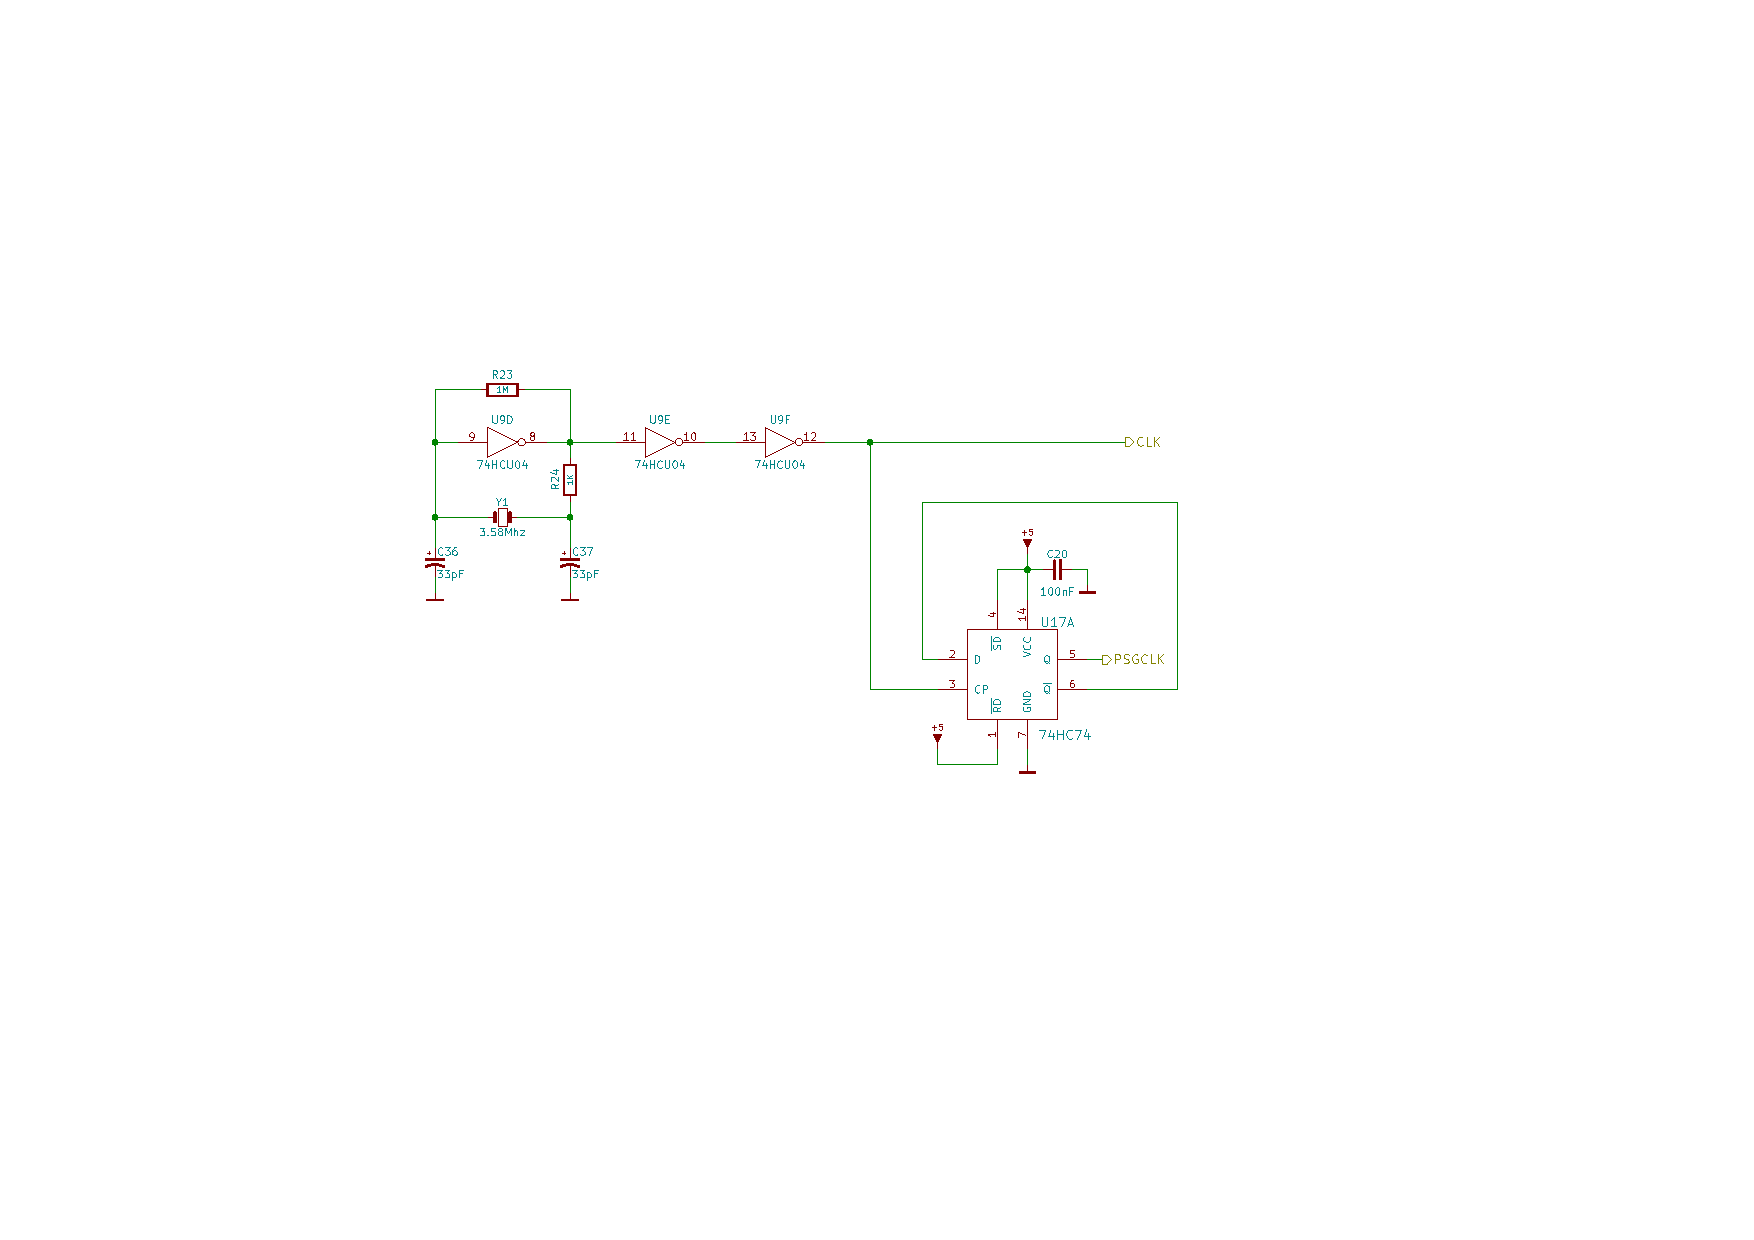
\includegraphics[width=\linewidth,trim={7cm 7.5cm 9cm 6cm},clip]{figures/artemisa-schematic-clock}
  \caption{Schematic diagram of clock generator}
  \label{fig:artemisa-schematic-clock}
\end{figure}

The clock generator is the circuit responsible of generating a squared clock signal. The clock signal is used by some devices such as the CPU or the PSG to synchronize their actions.

In fact, the circuit generates two different clock signals. One is {\tt CLK}, the system clock signal with a frequency of 3.58Mhz. The other is {\tt PSGCLK}, the clock signal used by the Programmable Sound Generator (PSG) in order to produce waveforms.

At the top-left side of the schematic we can see how {\tt CLK} is generated. The most important part of this design is the quartz crystal oscillator {\tt Y1}. This device will produce a